\documentclass{beamer}
\usetheme{CMU}

\usepackage{pgf,pgfarrows,pgfnodes,pgfautomata,pgfheaps,pgfshade}
\usepackage{amsmath,amssymb}
\usepackage[utf8]{inputenc}
\usepackage{colortbl}
\usepackage[english]{babel}
\usepackage{booktabs}
\usepackage{slpython}
\usepackage{underscore}

\author{Luís Pedro Coelho}
\institute{Programming for Scientists}

\graphicspath{{figures/}{figures/generated/}{images/}}

\newcommand*{\code}[1]{\textsl{#1}}


\title{Software Engineering}
\begin{document}
\frame{\maketitle}

\begin{frame}[fragile]
\frametitle{Software Engineering}
Most projects that we are tackling do not need software engineering.

\note{Still, some techniques are either useful by themselves or something you will learn about.}
\end{frame}

\begin{frame}[fragile]
\frametitle{Traditional Software Engineering}

\begin{block}{Waterfall Model}
\begin{enumerate}
\item Requirements
\item Design
\item Implementation
\item Testing
\item Maintenance
\end{enumerate}
\note{According to wikipedia, this was---from the start---presented as the *wrong* way to do things.}
\end{block}
\end{frame}

\begin{frame}[fragile]
\frametitle{Waterfall}

\centering
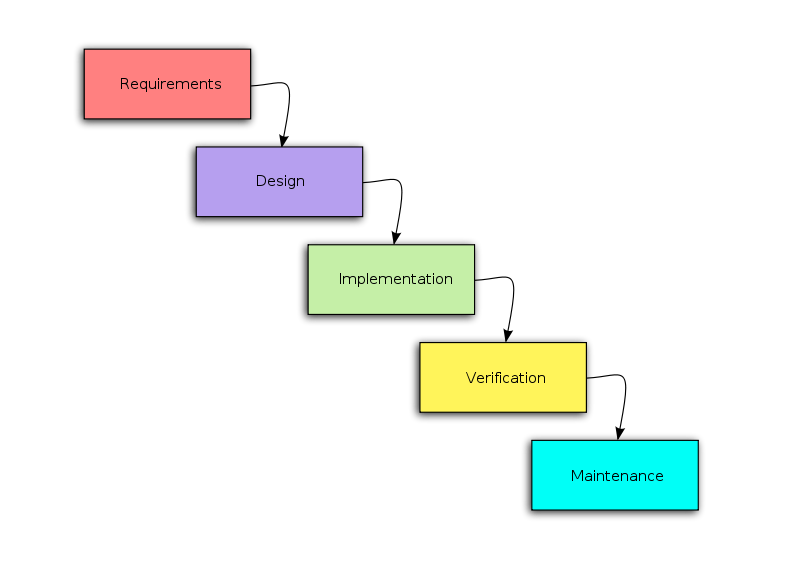
\includegraphics[width=.9\textwidth]{waterfall.png}

\note{(Wikipedia)}
\end{frame}

\begin{frame}[fragile]
\frametitle{Iterated Waterfall}

\begin{enumerate}
\item Requirements
\item Design
\item Implement
\item Testing
\item Maintenance
\item Goto 1
\end{enumerate}
\end{frame}

\begin{frame}[fragile]
\frametitle{Requirements for Particles}

\begin{block}{Major Goals}


\begin{itemize}
\item Implement particle simulation using \textit{Brownian} dynamics.
\item Generate a video containing shot noise.
\item Detect particles using global thresholding
\item Track using Hungarian algorithm
\item Compared inferred std.\ dev.\ with underlying std.\ dev.
\item \ldots
\end{itemize}
\end{block}
\begin{block}{Minor Goals}

\begin{itemize}
\item Allow the user to set the random seed.
\item Allow the user to save the video to a file.
\item \ldots
\end{itemize}
\end{block}
\end{frame}

\begin{frame}[fragile]
\frametitle{Design of Particles}

\begin{itemize}
\item List of tracks
\item Tracks
\item Video
\item Positions
\end{itemize}
\end{frame}

\begin{frame}[fragile]
\frametitle{Unified Modeling Language}

\centering
\includegraphics[width=.9\textwidth]{Track.png}

\note{I don't recommend full UML as it was intended to be used..

It's a good way to communicate with others or, in a much less formal version,
to think about the design.}
\end{frame}

\begin{frame}[fragile]
\begin{python}
class Track:
    def __init__(self) :
        self.positions = None # List<positions>
        self.start_time = None # int
        pass
class Position:
    def __init__(self) :
        pass
    def next (self, method) :
        pass # returns Position
class 2D Position (Position) :
    def __init__(self) :
        self.y = None # int
        self.x = None # int
        pass
    def next (self, method) :
        pass # returns position
\end{python}
\end{frame}

\begin{frame}[fragile]

\centering
\includegraphics[height=.8\textheight]{gentracks.png}

\end{frame}

\begin{frame}[fragile]
\frametitle{Design of Particles: Our Version}

\begin{itemize}
\item List of tracks: simple Python list
\item Tracks: $(t_0,[p_0,p_1,\cdots])$
\item Video: numpy 3-d array
\item position: class Position
\end{itemize}
\end{frame}


\begin{frame}[fragile]
\frametitle{Use Cases}
\begin{block}{Use Case 1}
Rita is a biologist. She does not care much about algorithms, but wants to know how
fast some particles move inside the cell. She has collected some images and applied
the Hungarian algorithm for tracking. Before publishing the results, she wants to have
validate her implementation. She manually tunes the parameters of the video until it looks 
like her real particles. She is computer savy, but does not know how to program.
\end{block}
\end{frame}

\begin{frame}[fragile]
\frametitle{Use Cases}
\begin{block}{Use Case 2}
Wang is a computer scientist. He is interested in testing his new fancy algorithm for
particle tracking and comparing it with the traditional Hungarian algorithm. He is confortable
with programming.
\end{block}
\end{frame}


\begin{frame}[fragile]
\frametitle{Agile Methodologies}

\begin{itemize}
\item Appeared in the mid-90's.
\item Focus on avoiding ``Big Design Up Front.''
\end{itemize}
\end{frame}

\begin{frame}[fragile]
\frametitle{Properties of Agile Methodologies}
\begin{itemize}
\item No big design up front.
\item Pair programming (two people programming at once). \note{Pair programming comes from a specific methodology called Xtreme Programming (XP)}
\item Test everything, test it twice.
\item Dynamic languages (Python, Ruby, Basic,\ldots).
\item Release early, release often.
\item Avoid over-engineering.
\item Organic growth instead of design.
\item Constant refactoring
\end{itemize}
\end{frame}

\begin{frame}[fragile]
\frametitle{Release Early, Release Often}

Short release cycles, even if internal.

\end{frame}

\begin{frame}[fragile]
\frametitle{Refactoring}

\begin{itemize}
\item Refactoring means \alert{improving the code}\\
    without \alert{changing the program}.
\item It often means paying down \alert{technical debt}
\end{itemize}

\end{frame}


\end{document}
